% =============================================================================
%  SoSa -- Sosyal Bilimler ve Sağlık Bülteni
%  Örnek makale / worked example for sosa.cls
%
%  Derleme / Compile:  pdfLaTeX, XeLaTeX veya LuaLaTeX -- iki kez (twice).
%  Overleaf: Menu > Compiler > pdfLaTeX (or XeLaTeX).
% =============================================================================
%
%  Sınıf seçenekleri / class options
%  ---------------------------------
%    ornament=alternate   şeritler bir sayfa atlayarak (varsayılan / default)
%    ornament=all         her sayfada şerit
%    ornament=none        şerit yok, tam genişlik metin
%    fontsize=11 | 12     gövde punto (varsayılan 11)
%    lang=turkish|english
%    ornamentfit=cover|stretch
%    proof                sayfa kılavuz çizgilerini göster
%
\documentclass[ornament=alternate,fontsize=11,lang=turkish]{sosa}

% -----------------------------------------------------------------------------
%  Sayfa süslemeleri / the right-hand ornament strips
% -----------------------------------------------------------------------------
% Şerit taşıyan sayfalarda sırayla kullanılacak görseller.
% The artwork used, in turn, on the pages that carry a strip.
\SosaOrnamentCycle{%
  assets/ornaments/ornament-01,%
  assets/ornaments/ornament-02,%
  assets/ornaments/ornament-03,%
  assets/ornaments/ornament-04,%
  assets/ornaments/ornament-05%
}

% Kapak bandı görseli / the hero band on the first page.
\SosaHero{assets/hero/hero-01}

% Belirli bir sayfaya belirli bir görsel:
%   \SosaOrnament{65}{assets/ornaments/ornament-03}
% Belirli sayfalarda şeridi kaldır:
%   \SosaNoOrnament{63,67}
% Belirli sayfalara şerit ekle:
%   \SosaForceOrnament{62}

% -----------------------------------------------------------------------------
%  Künye / running heads and pagination
% -----------------------------------------------------------------------------
\SosaStartPage{60}          % derginin sayfa numarası / first printed page
\SosaMasthead{Sosyal Bilimler ve Sağlık Bülteni (SoSa). 2026; Bahar(18):60-70}
\SosaRunningHead{Balıkesir'de Yaşayan Yetişkinlerin Sağlık Hizmetlerinde
  Yapay Zekâ Kullanımına Dair Görüşleri. SoSa. 2026;Bahar(18)}

% -----------------------------------------------------------------------------
%  Başlık sayfası / front matter
% -----------------------------------------------------------------------------
\SosaArticleType{Özgün Makale}

\SosaTitleTR{Balıkesir'de Yaşayan Yetişkinlerin Sağlık Hizmetlerinde
             Yapay Zekâ Kullanımına Dair Görüşleri}

\SosaTitleEN{Perspectives of Adults Living in Balıkesir on the Use of
             Artificial Intelligence in Healthcare}

% \sosaaff{n} = üst simge kurum numarası;  \orcid{...} = ORCID rozeti
\author{%
  Murat Aysin\sosaaff{1}\orcid{0000-0001-0000-0001},
  Sultan Eser\sosaaff{2}\orcid{0000-0001-0000-0002},
  Duygu Lüleci\sosaaff{1}\orcid{0000-0001-0000-0003},
  Emine Ayhan Akman\sosaaff{1}\orcid{0000-0001-0000-0004},
  Çağdaş Sonat\sosaaff{3}\orcid{0000-0001-0000-0005},
  Dursun Yasemin Yayla Keskin\sosaaff{3}\orcid{0000-0001-0000-0006},
  Alikemal Başol\sosaaff{3}\orcid{0000-0001-0000-0007},
  Ali Ceylan\sosaaff{4}\orcid{0000-0001-0000-0008}%
}

\SosaAffiliations{%
  \item Dr. Öğr. Üyesi, Balıkesir Üniversitesi, Tıp Fakültesi,
        Halk Sağlığı Anabilim Dalı. Balıkesir, Türkiye.
  \item Prof. Dr., Sağlık Bilimleri Üniversitesi, İzmir Tıp Fakültesi,
        Halk Sağlığı Anabilim Dalı, İzmir, Türkiye.
  \item Arş. Gör. Dr., Balıkesir Üniversitesi, Tıp Fakültesi,
        Halk Sağlığı Anabilim Dalı. Balıkesir, Türkiye.
  \item Prof. Dr., Balıkesir Üniversitesi, Tıp Fakültesi,
        Halk Sağlığı Anabilim Dalı. Balıkesir, Türkiye.%
}

\SosaOz{%
  \textbf{Giriş:} Yapay zekâ, sağlık hizmetlerinde tanı, tedavi planlaması,
  hastalık öngörüsü, hasta bakım yönetimi ve klinik karar destek süreçlerinde
  giderek daha fazla kullanım alanı bulmaktadır. Bu teknolojilerin sağlık
  sistemine başarılı biçimde entegre edilebilmesi, toplumun yapay zekâyı
  güvenilir ve faydalı bulmasıyla yakından ilişkilidir. Bu çalışmanın amacı,
  Balıkesir'de yaşayan yetişkinlerin sağlık hizmetlerinde yapay zekâ
  kullanımına dair görüşlerini belirlemektir.

  \textbf{Gereç-Yöntem:} Kesitsel tipteki çalışma, Temmuz 2024'te Balıkesir
  Altıeylül ilçesi merkez mahallelerinde yaşayan 18 yaş ve üzeri yetişkinlerde
  yürütüldü. Çok aşamalı küme örnekleme yöntemiyle 715 kişiye ulaşıldı.
  Veriler yüz yüze anket yöntemiyle Google Forms üzerinden toplandı. Veriler
  SPSS 26.0 programında analiz edildi; kategorik değişkenler için ki-kare;
  sürekli değişkenlerin analizi için t testi kullanıldı. Anlamlılık düzeyi
  p${<}$0,05 kabul edildi.

  \textbf{Bulgular:} Katılımcıların yaş ortalaması 40,3$\pm$15,3 olup
  \%52,9'u kadındı. Katılımcıların \%64,5'i yapay zekânın sağlık
  hizmetlerinde kullanımının faydalı olacağını düşünmekteydi. Katılımcıların
  \%44,8'i yapay zekânın doğru tanılar sunacağını düşünürken, \%57,3'ü
  kişisel verilerin güvenliği ile ilgili endişe duymaktaydı. Tek değişkenli
  analizlerde cinsiyet ve sağlık hizmetlerinde yapay zekânın kullanımında
  kişisel verilerin güvenliği ile ilgili endişe duyma dışında incelenen tüm
  değişkenler ile yapay zekâyı faydalı bulma durumu arasında anlamlı fark
  saptandı.

  \textbf{Sonuç-Öneriler:} Sağlık hizmetlerinde yapay zekâya yönelik fayda
  algısı sosyodemografik özellikler, sağlık durumu ve teletıp deneyimine göre
  değişmektedir. Toplumun farklı gruplarına yönelik güven temelli, anlaşılır
  ve kanıta dayalı bilgilendirme çalışmaları planlanmalıdır.%
}
\SosaKeywordsTR{sağlık hizmeti, yapay zeka, teletıp}

\SosaAbstract{%
  \textbf{Introduction:} Artificial intelligence is increasingly being used in
  healthcare, particularly in diagnosis, treatment planning, disease
  prediction, patient care management, and clinical decision support. The
  successful integration of these technologies into the healthcare system is
  closely associated with whether the public perceives artificial intelligence
  as reliable and beneficial. This study aimed to determine the views of
  adults living in Balıkesir regarding the use of artificial intelligence in
  healthcare.

  \textbf{Materials and Methods:} This cross-sectional study was conducted in
  July 2024 among adults aged 18 years and older living in the central
  neighborhoods of Altıeylül district, Balıkesir. A total of 715 participants
  were reached using multistage cluster sampling. Data were collected through
  face-to-face interviews using Google Forms. The data were analyzed using
  SPSS version 26.0. The chi-square test was used for categorical variables,
  and the t-test was used for continuous variables. Statistical significance
  was set at p${<}$0.05.

  \textbf{Results:} The mean age of the participants was 40.3$\pm$15.3 years,
  and 52.9\% were female. Overall, 64.5\% thought that artificial intelligence
  would be beneficial in healthcare. While 44.8\% believed that artificial
  intelligence would provide accurate diagnoses, 57.3\% expressed concerns
  about personal data security. In univariate analyses, all examined
  variables, except sex and concerns about personal data security, differed
  significantly according to whether artificial intelligence was perceived as
  beneficial.

  \textbf{Conclusion and Recommendations:} Perceptions of the benefits of
  artificial intelligence in healthcare vary according to sociodemographic
  characteristics, health status, and telemedicine experience. Clear,
  evidence-based, and trust-oriented informational activities should be
  planned for different groups in society.%
}
\SosaKeywordsEN{healthcare, artificial intelligence, telemedicine.}

% İsteğe bağlı: kongre bildirisi vb. notu / optional acknowledgement note
% \SosaNote{Bu makalede yer alan verilerin bir kısmı ... sunulmuştur.}

% -----------------------------------------------------------------------------
%  İlk sayfa künyesi / colophon at the foot of page one
% -----------------------------------------------------------------------------
\SosaReceived{16.05.2026}
\SosaAccepted{12.06.2026}
\SosaPublished{19.06.2026}
\SosaCorrespondingAuthor{Murat Aysin}
\SosaCorrespondingEmail{murat.aysin@balikesir.edu.tr}
\SosaHandlingEditor{Nuray Özgülnar}
\SosaCitation{Aysin, M., Eser, S., Lüleci, D., Ayhan Akman, E., Sonat, Ç.,
  Yayla Keskin, D. Y., Başol A., \& Ceylan A. (2026). Balıkesir'de Yaşayan
  Yetişkinlerin Sağlık Hizmetlerinde Yapay Zekâ Kullanımına Dair Görüşleri.
  \textit{Sosyal Bilimler ve Sağlık Bülteni (SoSa), BAHAR(18),} 60-70}

% =============================================================================
\begin{document}
\maketitle

\section{Giriş}

Yapay zekâ, insan zekâsını gerektiren öğrenme, akıl yürütme, problem çözme,
örüntü tanıma ve karar verme gibi bilişsel süreçlerin bilgisayar sistemleri
aracılığıyla gerçekleştirilebilmesini sağlayan teknolojileri ifade etmektedir.
Makine öğrenmesi, derin öğrenme ve doğal dil işleme alanlarındaki
gelişmelerle birlikte yapay zekâ, son yıllarda birçok alanda hızla
yaygınlaşmış; sağlık sektörü de bu dönüşümden en fazla etkilenen alanlardan
biri olmuştur (Fahim vd., 2025; OECD, 2024).

Sağlık hizmetlerinde yapay zekâ; tanı, tedavi planlaması, hastalık öngörüsü,
ilaç geliştirme, kişiselleştirilmiş sağlık hizmetleri, hasta bakım yönetimi ve
klinik karar destek süreçlerinde kullanılma potansiyeli taşımaktadır. Ayrıca
halk sağlığı alanında salgınların erken tespiti, risk gruplarının belirlenmesi
ve sağlık kaynaklarının planlanması gibi konularda önemli fırsatlar sunmaktadır
(Alum \& Ugwu, 2025; DSÖ, 2025; Kaplan vd., 2024; Panteli vd., 2025). Bu
gelişmeler sağlık hizmetlerinden yararlanan toplumun yapay zekâya ilişkin
beklenti ve güven düzeyini önemli hale getirmektedir. Çünkü sağlık
hizmetlerinde yapay zekâ kullanımının sürdürülebilirliği ve başarısı, toplum
katılımı ve toplumun bu uygulamaları benimsemesi ile yakından ilişkilidir
(Osnat, 2025).

Son yıllarda yapay zekâ alanındaki ilerlemeler toplumun dikkatini çekmiş,
yapay zekâ uygulamalarının yaygınlaşmasıyla halkın konuya ilgisi artmıştır. Bu
ilgi, sağlık hizmetlerinde yapay zekâ uygulamalarının olası yararlarına ilişkin
beklentileri artırırken, bu uygulamaların risklerine yönelik kaygıları da
beraberinde getirmektedir. Daha hızlı hizmet, doğru tanı ve kolay erişim
beklentileri olumlu yönde etkilerken; mahremiyet, veri güvenliği, hatalı karar
verme ve etik sorunlar da kaygı yaratabilmektedir (Beets vd., 2023; Gundlack
vd., 2025). Bu bağlamda çalışmanın amacı, Balıkesir'de yaşayan yetişkinlerin
sağlık hizmetlerinde yapay zekâ kullanımına dair görüşlerini belirlemektir.

\section{Gereç-Yöntem}

Kesitsel tipteki bu çalışma için, Temmuz 2024'te Balıkesir Altıeylül ilçesi
merkez mahallelerinde yaşayan 18 yaş ve üzeri yetişkinlerden veri toplandı.
Araştırmanın evrenini Balıkesir ili Altıeylül ilçesinde yaşayan 18 yaş ve üzeri
107.052 yetişkin oluşturdu. Örneklem büyüklüğü Epi Info 7.2 programı
kullanılarak; \%95 güven aralığı, \%5 hata payı, \%50 sıklık, 1,5 desen etkisi
ve \%20 yedek ile 702 kişi olarak hesaplandı ve çok aşamalı küme örnekleme
yöntemiyle 715 kişiye ulaşıldı. Her mahalle, birer küme kabul edilip
ulaşılması gereken kişiler mahalle nüfusuna göre tabakalandırıldı. Basit
rastgele yöntem ile sokaklar belirlendi ve ilgili sokaklardan dört hane
seçildi. Her haneden bir kişi çalışmaya dahil edildi.

Anket görüşmeleri yüz yüze gerçekleştirildi. Anket için kâğıt baskı yerine
Google Forms platformu kullanıldı. Anket formu araştırmacılar tarafından
literatür taranarak oluşturuldu. Anket formu sosyodemografik özellikler; sağlık
durumu, alışkanlıklar, davranışlar ve teletıp deneyimi ile sağlık
hizmetlerinde yapay zekâ kullanımına ilişkin görüşlerden oluşmaktadır.
Toplanan veriler SPSS 26.0 programıyla çözümlendi. Tanımlayıcı veriler sayı ve
yüzde ile sunuldu. Kategorik değişkenlerin analizi için ki-kare testi, sürekli
değişkenlerin analizi için t testi kullanılmıştır. İstatistiksel anlamlılık
düzeyi p${<}$0,05 kabul edildi. Etik kurul onayı; Balıkesir Üniversitesi
Sağlık Bilimleri Girişimsel Olmayan Araştırmalar Etik Kurulundan alındı
(25/06/2024 tarih 2024/95 sayılı izin).

\section{Bulgular}

Katılımcıların yaş ortalaması 40,3 $\pm$ 15,3 olup \%52,9'u kadın, \%54'ü 50
yaş altında, \%50,8'i evli ve \%54,4'ü önlisans ve üzeri öğrenim düzeyine
sahipti. Katılımcıların \%53,6'sı herhangi bir işte çalışmakta, \%82,8'inin
hane geliri yoksulluk sınırının altındaydı. Katılımcıların sosyodemografik
özellikleri, sağlık durumları ve teletıp deneyimi ile ilgili bilgiler
Tablo~\ref{tab:sosyodemografik}'de sunulmuştur.

% -----------------------------------------------------------------------------
%  GENİŞ TABLO / a wide table
%  sosawide, sağdaki süsleme payını geri alır ve o sayfanın şeridini kaldırır.
%  sosawide reclaims the ornament reserve and drops that page's strip.
%  (İki kez derleyin / needs two compiles.)
% -----------------------------------------------------------------------------
\begin{table}[!ht]
\begin{sosawide}
\caption{Katılımcıların Sosyodemografik Özellikleri, Sağlık Durumu ve
         Teletıp Deneyimi}
\label{tab:sosyodemografik}
\centering
\begin{sosatabular}[\sosatablesmall]{@{}L{150pt}L{130pt}R{110pt}@{}}
\textbf{Değişkenler} &                    & \textbf{Sayı (\%)}    \\
\midrule
Yaş\textsuperscript{*} &                   & 40,3 $\pm$ 15,3       \\
\addlinespace[2pt]
\multirow{2}{*}{Yaş}   & 50 yaş altı       & 386 (\%54,0)          \\
                       & 50 yaş ve üzeri   & 329 (\%46,0)          \\
\addlinespace[2pt]
\multirow{2}{*}{Cinsiyet} & Erkek          & 337 (\%47,1)          \\
                       & Kadın             & 378 (\%52,9)          \\
\addlinespace[2pt]
\multirow{2}{*}{Medeni durum} & Bekar      & 352 (\%49,2)          \\
                       & Evli              & 363 (\%50,8)          \\
\addlinespace[2pt]
\multirow{2}{*}{Eğitim düzeyi} & Lise ve altı & 326 (\%45,6)       \\
                       & Önlisans ve üzeri & 389 (\%54,4)          \\
\addlinespace[2pt]
\multirow{2}{*}{Meslek} & Çalışmıyor       & 332 (\%46,4)          \\
                       & Çalışıyor         & 383 (\%53,6)          \\
\addlinespace[2pt]
\multirow{2}{*}{Hane geliri} & Yoksulluk sınırının altı & 592 (\%82,8) \\
                       & Yoksulluk sınırı ve üzeri & 123 (\%17,2) \\
\addlinespace[2pt]
\multirow{2}{*}{Çocuk varlığı} & Evet      & 393 (\%55,0)          \\
                       & Hayır             & 322 (\%45,0)          \\
\addlinespace[2pt]
\multirow{2}{*}{Kronik hastalık} & Evet    & 254 (\%35,5)          \\
                       & Hayır             & 461 (\%64,5)          \\
\addlinespace[2pt]
\multirow{2}{*}{İlaç kullanımı} & Evet     & 249 (\%34,8)          \\
                       & Hayır             & 466 (\%65,2)          \\
\addlinespace[2pt]
\multirow{2}{*}{Teletıp deneyimi varlığı} & Evet & 140 (\%19,6)    \\
                       & Hayır             & 575 (\%80,4)          \\
\end{sosatabular}

\vspace{2pt}
{\sosatablesmall \textsuperscript{*}Ortalama $\pm$ standart sapma}
\end{sosawide}
\end{table}

Katılımcıların \%64,5'i yapay zekânın tıpta faydalı olacağını düşünmekteydi.
\%44,8'i tıpta yapay zekânın doğru tanılar sunacağını düşünmekte ve \%57,3'ü
tıpta yapay zekâ kullanımında, kişisel verilerin güvenliği ile ilgili endişe
duymaktaydı. Katılımcıların sağlık hizmetlerinde yapay zekâ kullanımına
ilişkin bazı görüşleri Tablo~\ref{tab:gorusler}'de sunulmuştur.

% -----------------------------------------------------------------------------
%  NORMAL GENİŞLİKTE TABLO / a table that fits the ornament measure
% -----------------------------------------------------------------------------
\begin{table}[!ht]
\caption{Katılımcıların Sağlık Hizmetlerinde Yapay Zekâ Kullanımına İlişkin
         Bazı Görüşleri}
\label{tab:gorusler}
\begin{sosatabular}{@{}L{170pt}L{90pt}R{140pt}@{}}
\textbf{Değişkenler} & & \textbf{Sayı (\%)} \\
\midrule
\multirow{2}{170pt}{Sağlık hizmetlerinde yapay zekâ kullanımının faydalı
  olacağını düşünme}
                  & Evet     & 461 (\%64,5) \\
                  & Hayır    & 254 (\%35,5) \\
\addlinespace[4pt]
\multirow{3}{170pt}{Sağlık hizmetlerinde yapay zekânın doğru tanı sunacağını
  düşünme}
                  & Evet     & 320 (\%44,8) \\
                  & Kararsız & 248 (\%34,7) \\
                  & Hayır    & 147 (\%20,5) \\
\addlinespace[4pt]
\multirow{3}{170pt}{Sağlık hizmetlerinde yapay zekâ kullanımında kişisel
  verilerin güvenliği ile ilgili endişe duyma}
                  & Evet     & 410 (\%57,3) \\
                  & Kararsız & 196 (\%27,4) \\
                  & Hayır    & 109 (\%15,2) \\
\end{sosatabular}
\end{table}

Tablo~\ref{tab:gorusler}, sağlık hizmetlerinde yapay zekâ kullanımının faydalı
olacağını düşünen ve düşünmeyen bireylerin görüşlerini göstermektedir. Sağlık
hizmetlerinde yapay zekâ kullanımının faydalı olacağını düşünen bireylerin yaş
ortalaması (37,2 $\pm$ 14,4) düşünmeyenlere (45,7 $\pm$ 15,5) göre daha
düşüktü. Faydalı olacağını düşünme oranı 50 yaş altındakilerde \%73,8 iken,
50 yaş ve üzerindekilerde \%53,5'tir.

% -----------------------------------------------------------------------------
%  GÖRSEL / a figure
% -----------------------------------------------------------------------------
\begin{figure}[!ht]
  \centering
  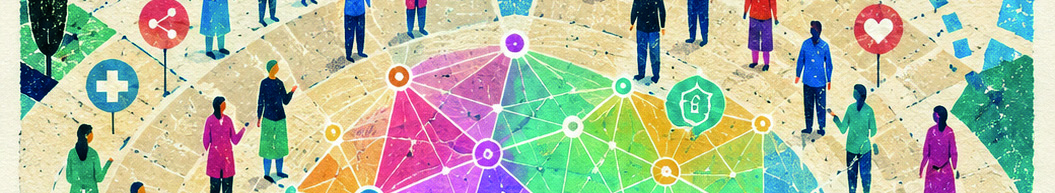
\includegraphics[width=0.62\textwidth]{assets/hero/hero-01}
  \caption{Yapay zekâya yönelik fayda algısının yaş gruplarına göre dağılımı}
  \label{fig:fayda}
\end{figure}

\section{Tartışma}

Bu çalışmada Balıkesir'de yaşayan yetişkinlerin yaklaşık üçte ikisinin sağlık
hizmetlerinde yapay zekâ kullanımını faydalı bulduğu saptanmıştır. Bu oran,
literatürdeki toplum tabanlı çalışmalarla benzerlik göstermektedir
(Aras vd., 2025; Busch vd., 2025). Bununla birlikte katılımcıların yarısından
fazlasının kişisel verilerin güvenliğine ilişkin endişe taşıması, mahremiyetin
kabul sürecindeki belirleyici rolüne işaret etmektedir
(Atalay \& Yücel, 2024; Esmaeilzadeh vd., 2021).

\begin{quote}
Alan yazında dijital sağlık uygulamalarının benimsenmesinde güvenin, algılanan
faydadan bağımsız biçimde belirleyici olduğu, özellikle veri paylaşımı söz
konusu olduğunda öne çıktığı bildirilmektedir.
\end{quote}

Çalışmanın Balıkesir ili Altıeylül ilçesi merkez mahallelerinde yürütülmüş
olması, bulguların diğer yerleşim yapılarına genellenebilirliğini
sınırlayabilir. Buna karşın çalışmanın toplum tabanlı olması ve yapay zekâya
yönelik fayda algısını sosyodemografik özelliklerle birlikte değerlendirmesi
önemli bir güçlü yönüdür.

\section{Sonuç ve Öneriler}

Sağlık hizmetlerinde yapay zekâya yönelik fayda algısı sosyodemografik
özellikler, sağlık durumu ve teletıp deneyimine göre değişmektedir. Toplumun
farklı gruplarına yönelik güven temelli, anlaşılır ve kanıta dayalı
bilgilendirme çalışmaları planlanmalıdır.

% -----------------------------------------------------------------------------
%  KAYNAKLAR / references -- APA 7, asılı girinti / hanging indent
%  Girdileri boş satırla ayırın. Separate entries with a blank line.
% -----------------------------------------------------------------------------
\begin{sosareferences}

Alum, E. U., \& Ugwu, O. P.-C. (2025). Artificial intelligence in disease
diagnosis and treatment. \textit{Discover Applied Sciences, 7}(3), 193.
\url{https://doi.org/10.1007/s42452-025-06616-y}

Aras, S., Drakos, C., Manimangalam, V., \& Nasir, M. A. (2025). Public
acceptance of artificial intelligence (AI) in healthcare.
\textit{Frontiers in Digital Health, 7}, 1664345.
\url{https://doi.org/10.3389/fdgth.2025.1664345}

Atalay, H. N., \& Yücel, Ş. (2024). Decoding privacy concerns in health data
disclosure. \textit{Archives of Public Health, 82}(1), 189.
\url{https://doi.org/10.1186/s13690-024-01416-z}

Beets, B., Newman, T. P., Howell, E. L., Bao, L., \& Yang, S. (2023).
Surveying public perceptions of artificial intelligence in health care in the
United States: Systematic review. \textit{Journal of Medical Internet
Research, 25}(1), e40337. \url{https://doi.org/10.2196/40337}

Esmaeilzadeh, P., Mirzaei, T., \& Dharanikota, S. (2021). Patients' perceptions
toward human--artificial intelligence interaction in health care: Experimental
study. \textit{Journal of Medical Internet Research, 23}(11), e25856.
\url{https://doi.org/10.2196/25856}

\end{sosareferences}

\end{document}
